\subsection{Real LLM on real MMLU-Pro (T1)}
\label{sec:t1}
\textbf{Design.} The system is Qwen2.5-1.5B-Instruct~\citep{qwen2024qwen25} (Q8\_0 GGUF, llama.cpp, CPU; Apache-2.0) answering MMLU-Pro~\citep{wang2024mmlupro} (pinned revision, MIT license, 10 options) by reading out the log-probabilities of the ten option letters. The configuration family has 24 base prompts (4 instruction styles $\times$ 2 answer cues $\times$ \{0-shot, two 3-shot demonstration sets from the validation split\}) plus the 276 two-prompt logit-average ensembles of them as a pipeline-like extension: $K_{\max}=300$ candidates. All 300 are scored once on a fixed pool of 2000 randomly drawn test questions and the per-item outcomes are cached; a search is then \emph{replayed}: draw a search set $D$ of $n$ pool items, let the procedure choose $\hatc$ among $K$ candidates (the baseline prompt plus $K-1$ random ones; $K=24$ is the base family), and score $\hatc$ on the remaining pool items minus a left-out block (1300--1750 fresh items, binomial SE $\approx$1.1--1.3 points, independent of the search). The pool accuracies of the 24 base prompts range from 20.5\% to 29.2\% and the best of all 300 is 30.1\%; the between-candidate spread is small ($\tau\approx0.017$--$0.024$ on the probability scale) and candidates are strongly correlated (binary item correlation 0.57--0.68). The baseline prompt has 22.7\%. 52 replay cells with 1000 replicates each; because replicates share the fixed pool, every uncertainty in this subsection is $\pm1.96\times$ a delete-a-block SE (10 blocks of replicates) rather than a replicate SE or Wilson interval; it reflects the variation over search sets given the pool, not the uncertainty about the pool itself, which we do not estimate.

\textbf{Gap.} (Fig.~\ref{fig:A1}.) The naive report is optimistic here too. For $K=300$ and $n=100$ the selected configuration is reported at 33.7\% and scores 28.0\% on fresh items: a 5.7-point gap (block SE 0.11). Against the baseline's 22.7\%, the reported improvement is 11.0 points while the real one is 5.3: about twice as large. The gap is 8.7 points at $n=50$ and 1.9 at $n=500$ ($K=300$), and 4.6 points for the 24 base prompts alone ($n=100$). It grows with $K$ and falls with $n$ like the extreme-value formula evaluated with the matrix's own $(\sigma,r,\tau)$, which is within 0.51 points of every one of the 35 exhaustive cells (mean difference $-0.04$ points), although 13 of the 35 differ by more than 1.96 block SE, mostly at small $K$ and $n=50$ where it over-predicts (e.g.\ $K=2$, $n=50$: 1.80 predicted, 1.29 observed). The parameters are estimated from the same matrix, so this checks the functional form, not a held-out prediction. The synthetic grid of T0 gives a larger gap than the real one in 28 of its 30 nearest cells (median ratio 1.6; its correlation grid does not contain the matrix's), so we treat T0 as a model of the mechanism, not a calibrated replica (Fig.~\ref{fig:T1check}, appendix). Halving and greedy search are mildly less optimistic than exhaustive search (4.0 and 4.1 vs.\ 4.5 points at $n=100$, $K=24$; 5.2 vs.\ 5.7 at $K=300$). The gap is present in every one of the 14 MMLU-Pro subjects (3.3 to 7.0 points at $n=100$, $K=24$; Fig.~\ref{fig:T1subj}, appendix).

\textbf{Reporting methods and decisions.} (Table~\ref{tab:G}.) The naive interval covers $\theta(\hatc)$ in 77.1 $\pm$ 3.2\% ($n=100$) and 80.6 $\pm$ 2.2\% ($n=500$; $\pm1.96$ block SE) of replicates at $K=300$ and is biased by $+5.7$ and $+1.9$ points. Hold-out (M1, 0.95/0.94 at half split), the hybrid conditional interval (0.953/0.935) and cross-fitting (0.92/0.88) are close to nominal and unbiased; the conditional interval is nominal but its point estimate is heavy-tailed (RMSE 20.8 points at $n=100$); the simultaneous bound is conservative (0.988) and as biased as M0; the empirical-Bayes interval again fails (0.11/0.22). Bootstrap optimism correction removes most but not all of the bias ($+1.8$ points at $n=100$, $K=300$, vs.\ $+5.7$ for M0; appendix). Because the 276 ensembles are not independent systems and the candidates differ little, "tuned beats baseline" is almost always true here, so false-claim rates are not identifiable from these cells; we use a paired design instead (Table~\ref{tab:H}): two systems tuned with $K_A=75$ and $K_B=5$ candidates on the same $n=100$ items, where the true difference is on average 0.5 points and A is truly better in only 61.7\% of the replicates. Naive reports declare A better in 90.3\% of replicates (the reported difference is $+3.0$ points against a true $+0.5$); among the 383 replicates in which A is not truly better, 87.5\% still call it better with M0, versus 43--56\% for hold-out, cross-fitting and the selection-aware point rules. With a rule that requires A's 95\% lower bound to exceed B's estimate the false-winner rate is 0\% for M0 and the simultaneous bound and 3.1--3.4\% for hold-out, cross-fitting and the conditional/hybrid intervals, but those rules detect a truly better A in only 7--9\% of replicates (M0: 1.8\%); the equal-$K$ pairs have no true difference, and every report order there is a coin flip (flip rates near 0.5 by construction).

\begin{figure}[t]
\centering
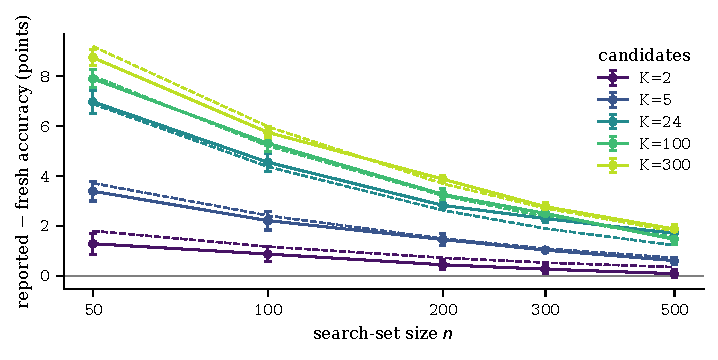
\includegraphics[width=\linewidth]{fig_a_t1.pdf}
\caption{\textbf{Optimism of the naive report on the real outcome matrix (T1).} Reported minus fresh-item accuracy of the selected configuration against $n$, for $K$ candidates searched exhaustively (Qwen2.5-1.5B-Instruct, MMLU-Pro; 1000 replicates per cell). Bars: mean $\pm1.96\times$ delete-a-block SE (replicates share one 2000-item pool, so the replicate SE is too small); dashed: the closed form fed with the matrix's own $(\sigma,r,\tau)$.}
\label{fig:A1}
\end{figure}

\begin{table}[t]
\caption{\textbf{Calibration of reporting methods on the real matrix (T1), $K=300$, $n=100$, 1000 replicates} ($n=500$ in the appendix). Bias and RMSE in points against each method's own target; coverage $\pm1.96$ block SE; median width (points); items used for the report.}
\label{tab:G}
\centering\scriptsize
\resizebox{\linewidth}{!}{\input{../tables/table_g_main.tex}}
\end{table}

\begin{table}[t]
\caption{\textbf{Ranking two tuned systems on the same search set (T1).} A and B are tuned exhaustively from disjoint candidate subsets of $K_A$ and $K_B$ configurations; 1000 replicates per cell, $\pm1.96$ block SE. Flip: the reported order differs from the true order (a tie counts as a flip). The 75 vs.\ 5 pair has the largest search-effort contrast; the equal-$K$ pairs are controls with no true difference.}
\label{tab:H}
\centering\scriptsize
\resizebox{\linewidth}{!}{\input{../tables/table_h_t1_pairs.tex}}
\end{table}
